% ============================================================================
% Geospatial World Modeling via Frozen Foundation Model Embeddings
% and Lightweight Latent Dynamics
% ============================================================================
% Target journal: International Journal of Geographical Information Science
% (Taylor & Francis)
% ============================================================================
\documentclass{article}

\usepackage{amsmath,amssymb}
\usepackage{booktabs}
\usepackage{graphicx}
\usepackage{multirow}
\usepackage{caption}
\usepackage{subcaption}
\usepackage{algorithm}
\usepackage{algorithmic}
\usepackage{hyperref}
\usepackage{color}
\usepackage{natbib}
\usepackage{tikz}
\usetikzlibrary{positioning,arrows.meta,shapes.geometric,fit,calc}
\graphicspath{{./figures/}{./}}
\bibliographystyle{plainnat}

\begin{document}

\makeatletter
\@ifundefined{ANONYMIZE}{
  \title{Geospatial World Modeling via Frozen Foundation Model Embeddings and Lightweight Latent Dynamics}
  \author{Ning Zhou$^{a}$ and Xiang Jing$^{a}$$^{\ast}$\thanks{$^\ast$Corresponding author. Email: jingxiang@pku.edu.cn}\\
  $^{a}${\em School of Software and Microelectronics, Peking University, Beijing 100871, China}}
}{
  \title{Geospatial World Modeling via Frozen Foundation Model Embeddings and Lightweight Latent Dynamics}
  \author{Anonymous authors}
}
\makeatother

\date{}
\maketitle

\begin{abstract}
Predicting land-use and land-cover (LULC) change is fundamental to geographic information science, yet existing methods either operate on discrete categorical maps or require prohibitively large pixel-level generative models. We propose a geospatial world model that predicts LULC change entirely within a learned embedding space, following the Joint Embedding Predictive Architecture (JEPA) paradigm. Our approach combines a frozen geospatial foundation model---AlphaEarth Foundations (480M+ parameters)---producing 64-dimensional per-pixel embeddings, with a lightweight \textit{LatentDynamicsNet} (459K parameters) that learns residual state transitions via autoregressive rollout. Three technical contributions enable this: (1) explicit L2 re-normalization to prevent manifold drift on the unit hypersphere; (2) dilated convolutions expanding the receptive field to 170\,m for macro-scale drivers; and (3) multi-step unrolled training loss to mitigate exposure bias. Ablation confirms all three are critical: removing L2 normalization degrades advantage by 62\%, dilated convolutions by 32\%, and unrolled loss turns validation negative. Experiments span 17 study areas across China with strict train/val/test/OOD splits, evaluated against persistence and linear extrapolation baselines. The model achieves mean cosine similarity of 0.9575, surpassing persistence (0.9460) on all 12 training areas. On pixels undergoing actual change, advantage amplifies to $+0.030$--$+0.108$. Multi-step rollout sustains above-baseline quality for up to 6 steps. These results demonstrate that frozen foundation model embeddings provide a viable state space for geospatial world modeling with three orders of magnitude fewer parameters than comparable models.
\end{abstract}

\begin{keywords}
geospatial world model; JEPA; foundation model embeddings; land-use change prediction; latent dynamics; AlphaEarth
\end{keywords}

% ============================================================================
\section{Introduction}
\label{sec:intro}
% ============================================================================

Predicting how land surfaces will change over time is a central problem in geographical information science, with direct applications in urban planning, agricultural policy, ecological conservation, and climate adaptation \citep{verburg2004lulc}. Traditional approaches---cellular automata--Markov chains (CA-Markov), CLUE-S, and logistic regression---operate on categorical land-use maps, relying on hand-calibrated transition probabilities and socioeconomic driving factors \citep{veldkamp2004clues}. While effective in constrained scenarios, these methods cannot capture the rich, continuous spectral--spatial--temporal information present in modern satellite observations.

Recent advances in deep learning have introduced more powerful alternatives. Convolutional--recurrent architectures (ConvLSTM) can learn spatiotemporal patterns from classified imagery sequences \citep{shi2015convlstm}. EarthPT \citep{smith2023earthpt}, a 700M-parameter autoregressive transformer, predicts pixel-level spectral reflectance forward in time. DiffusionSat \citep{khanna2023diffusionsat} uses conditional diffusion models to generate future satellite images. However, all of these operate in raw observation space (spectral bands or classified pixels), inheriting two fundamental limitations: (1) prediction in high-dimensional pixel space is computationally expensive and prone to hallucination artifacts; and (2) pixel-level prediction conflates semantically meaningful change with irrelevant noise (cloud shadows, atmospheric variation, sensor calibration drift).

In the broader AI community, the concept of a \textit{world model}---a learned internal simulator that predicts environment state transitions in a compressed latent space---has emerged as a powerful paradigm for planning and reasoning. Pioneered by \citet{ha2018world} and advanced through the Dreamer family \citep{hafner2023dreamerv3} and MuZero \citep{schrittwieser2020muzero}, world models separate perception (encoding observations into latent states) from dynamics (predicting latent state transitions), enabling efficient forward simulation without rendering full observations. LeCun's JEPA framework \citep{lecun2022jepa} formalizes this principle: predict in representation space, not pixel space.

Simultaneously, geospatial foundation models (GeoFMs) have made pre-trained, high-quality representations of the Earth's surface freely available. AlphaEarth Foundations \citep{brown2025alphaearth} produces 64-dimensional L2-normalized embedding vectors at 10\,m resolution for every land pixel on Earth, annually from 2017 to 2024, derived from multi-sensor inputs (Sentinel-1/2, Landsat, GEDI, ERA5) via a 480M+ parameter vision transformer. These embeddings have been shown to be physically interpretable \citep{rahman2026interpretable} and linearly decodable to land-cover classes with $>$83\% accuracy.

This paper bridges these two developments: we treat GeoFM embeddings as the state space of a geospatial world model. Our key insight is that if a foundation model has already learned to compress satellite observations into semantically meaningful, temporally varying embeddings, then the dynamics of land-use change can be learned \textit{on top of} these frozen embeddings using a lightweight neural network---without retraining the foundation model and without ever generating pixel-level predictions. This corresponds precisely to the JEPA architecture: the foundation model serves as the encoder; a small LatentDynamicsNet serves as the predictor.

To our knowledge, this is the first work to combine frozen geospatial foundation model embeddings with a learned dynamics model for autoregressive land-use change prediction. The closest prior works either train their own encoder end-to-end (MM-VSF, \citealt{mmvsf2024}), operate in spectral space with vastly larger models (EarthPT), or predict downstream variables rather than the embeddings themselves (PDFM+TimesFM, \citealt{google2024pdfm}).

Our contributions are:

\begin{enumerate}
\item We formulate geospatial world modeling as residual dynamics learning in a frozen GeoFM embedding space, and demonstrate its feasibility through a three-phase validation pipeline (signal verification, temporal holdout, spatial generalization).

\item We design the \textit{LatentDynamicsNet}, a 459K-parameter dilated convolutional network with L2 manifold preservation, scenario conditioning, and terrain context inputs, achieving meaningful prediction with 1{,}500$\times$ fewer parameters than EarthPT.

\item We introduce multi-step unrolled training loss to combat exposure bias, extending the effective prediction horizon from 1--3 years to 5+ years on training domains.

\item We provide comprehensive experiments on 17 Chinese study areas with strict train/val/test/OOD splits, two baselines, and a novel change-pixel evaluation protocol that reveals model advantages masked by globally dominant stable pixels.
\end{enumerate}


% ============================================================================
\section{Related Work}
\label{sec:related}
% ============================================================================

\subsection{LULC change prediction}

LULC change prediction has evolved from statistical models to deep learning approaches. CA-Markov \citep{veldkamp2004clues} combines cellular automata neighborhood rules with Markov chain transition matrices. CLUE-S \citep{verburg2002clues} incorporates logistic regression with socioeconomic drivers. More recently, Themeda \citep{turnbull2025themeda} uses ConvLSTM with 33 years of data and auxiliary climate variables, achieving 93.4\% pixel-wise accuracy for FAO Level 3 classes. TAMMs \citep{guo2025tamms} unifies temporal change description with future satellite image generation via MLLM and diffusion models.

\subsection{Earth observation foundation models}

GeoFMs have rapidly advanced. Prithvi-EO-2.0 \citep{jakubik2024prithvi} provides multi-temporal embeddings for classification tasks. SatMAE \citep{cong2022satmae} uses masked autoencoders with temporal positional encoding. Clay and Presto offer alternative embedding approaches. AlphaEarth Foundations \citep{brown2025alphaearth} stands out by providing annually-resolved, globally-available, 64-dimensional embeddings at 10\,m resolution through Google Earth Engine, with demonstrated physical interpretability \citep{rahman2026interpretable, benavides2026whatonearth}.

\subsection{World models and JEPA}

World models originated in reinforcement learning: Ha \& Schmidhuber's ``World Models'' \citep{ha2018world} learn compressed environment dynamics for policy training. Dreamer V3 \citep{hafner2023dreamerv3} achieves human-level performance across diverse domains using Recurrent State-Space Models (RSSMs). LeCun's JEPA \citep{lecun2022jepa} formalizes the principle of predicting in representation space rather than pixel space. AnySat \citep{astruc2024anysat} applies JEPA to remote sensing but for spatial mask prediction, not temporal dynamics. RemoteBAGEL \citep{remotebagel2025} proposes spatial extrapolation (generating adjacent tiles) but not temporal forecasting.

\subsection{Closest prior work}

MM-VSF \citep{mmvsf2024} predicts future satellite embeddings from current ones but trains its own encoder end-to-end rather than using a frozen foundation model. EarthPT \citep{smith2023earthpt} performs autoregressive prediction on raw spectral reflectance with 700M parameters. PDFM+TimesFM \citep{google2024pdfm} uses geospatial embeddings with a forecasting model but predicts socioeconomic variables, not the embeddings themselves. Our approach is the first to learn autoregressive dynamics \textit{on top of frozen GeoFM embeddings}.


% ============================================================================
\section{Study Areas and Data}
\label{sec:data}
% ============================================================================

\subsection{Study areas}

We select 17 study areas across China, covering four major land-type categories, with a strict four-way split to evaluate generalization (Table~\ref{tab:areas}). Each area spans approximately 0.1\textdegree$\times$0.1\textdegree\ ($\approx$10\,km$\times$10\,km) at 10\,m resolution.

\begin{table}[htbp]
\centering
\caption{Study areas by split and land-type category.}
\label{tab:areas}
\begin{tabular}{llll}
\toprule
Split & Area name & Category & Bbox (WGS84) \\
\midrule
\multirow{12}{*}{Train (12)} & Yangtze Delta & Urban & [121.2, 31.0, 121.3, 31.1] \\
 & Jing-Jin-Ji & Urban & [116.3, 39.8, 116.4, 39.9] \\
 & Chengdu Plain & Urban & [104.0, 30.6, 104.1, 30.7] \\
 & NE Plain & Agriculture & [126.5, 45.7, 126.6, 45.8] \\
 & N.~China Plain & Agriculture & [115.0, 36.5, 115.1, 36.6] \\
 & Jianghan Plain & Agriculture & [113.5, 30.3, 113.6, 30.4] \\
 & Hetao & Agriculture & [107.0, 40.7, 107.1, 40.8] \\
 & Yunnan Eco & Ecology & [100.2, 25.0, 100.3, 25.1] \\
 & Daxinganling & Forest & [124.0, 50.3, 124.1, 50.4] \\
 & Qinghai Edge & Plateau & [101.5, 36.5, 101.6, 36.6] \\
 & Guanzhong & Mixed & [108.9, 34.2, 109.0, 34.3] \\
 & Minnan Coast & Mixed & [118.0, 24.4, 118.1, 24.5] \\
\midrule
\multirow{2}{*}{Val (2)} & Pearl River & Urban & [113.2, 23.0, 113.3, 23.1] \\
 & Poyang Lake & Wetland & [116.0, 29.0, 116.1, 29.1] \\
\midrule
Test (1) & Wuyi Mountain & Forest & [117.6, 27.7, 117.7, 27.8] \\
\midrule
\multirow{2}{*}{OOD (2)} & Sanxia Reservoir & Mixed & [110.3, 30.8, 110.4, 30.9] \\
 & Lhasa Valley & Plateau & [91.1, 29.6, 91.2, 29.7] \\
\bottomrule
\end{tabular}
\end{table}

\subsection{Data sources}

\textbf{AlphaEarth Embeddings.} We use the \texttt{GOOGLE/SATELLITE\_EMBEDDING/V1/ANNUAL} dataset on Google Earth Engine (GEE), which provides 64-dimensional L2-normalized embedding vectors at 10\,m resolution for each year from 2017 to 2024. For each study area and year, 500 random pixel locations are sampled using \texttt{ee.Image.sample()} with \texttt{seed=42} for reproducibility, yielding $500\times64$ embedding matrices. All raw data are cached locally as NumPy \texttt{.npy} files for offline reproducibility.

\textbf{LULC Labels.} Land-cover class labels for decoder training are obtained from the ESRI Global LULC 10\,m Time Series (\texttt{projects/sat-io/open-datasets/landcover/ESRI\_Global-LULC\_10m\_TS}) on GEE, providing 9 land-cover classes at matching spatial resolution.

\textbf{Terrain Context.} DEM elevation and slope are derived from SRTM 30\,m (\texttt{USGS/SRTMGL1\_003}) via GEE. Elevation is min-max normalized to $[0,1]$; slope is clipped and normalized by 45\textdegree.


% ============================================================================
\section{Methodology}
\label{sec:method}
% ============================================================================

\subsection{Architecture overview}

Our system follows a two-layer architecture (Fig.~\ref{fig:architecture}):

\begin{itemize}
\item \textbf{Layer 1: Frozen encoder.} AlphaEarth Foundations (480M+ parameters) maps satellite observations to 64-dimensional unit vectors. This layer is never trained; we consume its outputs as pre-computed embeddings.
\item \textbf{Layer 2: Learned dynamics.} LatentDynamicsNet (459K parameters) predicts the next year's embedding given the current embedding, a scenario encoding, and optional terrain context.
\end{itemize}

This corresponds to the JEPA framework \citep{lecun2022jepa}: the encoder produces representations; the predictor operates in representation space. The decoder (a linear classifier) is used only for visualization, not during dynamics prediction.

\begin{figure}[htbp]
\centering
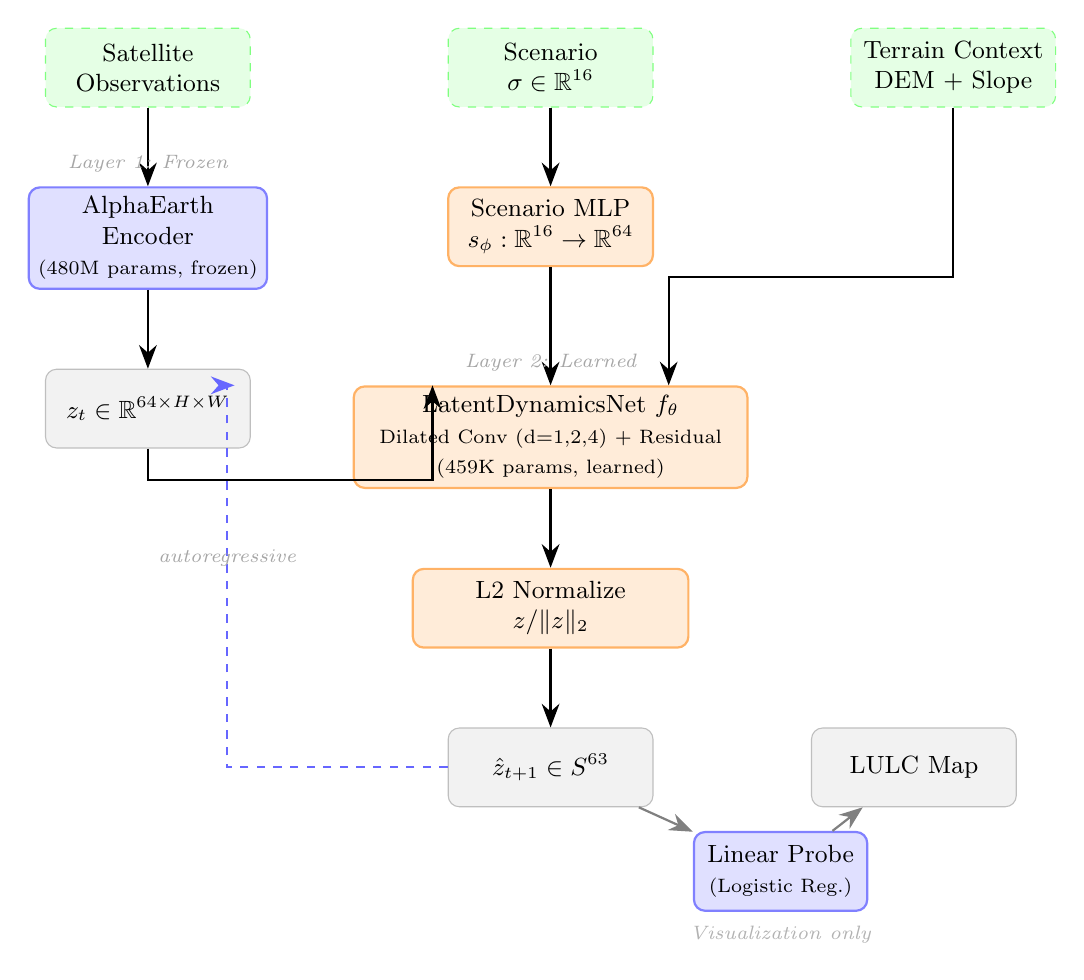
\begin{tikzpicture}[
    node distance=1.2cm and 1.8cm,
    box/.style={draw, rounded corners, minimum height=1.0cm, minimum width=2.6cm, align=center, font=\small},
    frozen/.style={box, fill=blue!12, draw=blue!50, thick},
    learned/.style={box, fill=orange!15, draw=orange!60, thick},
    input/.style={box, fill=green!10, draw=green!50, dashed},
    output/.style={box, fill=gray!10, draw=gray!50},
    arr/.style={-{Stealth[length=3mm]}, thick},
    label/.style={font=\scriptsize\itshape, text=gray!70},
]

% Row 1: Inputs
\node[input] (sat) {Satellite\\Observations};
\node[input, right=2.5cm of sat] (scenario) {Scenario\\$\sigma \in \mathbb{R}^{16}$};
\node[input, right=2.5cm of scenario] (terrain) {Terrain Context\\DEM + Slope};

% Row 2: Encoder + Scenario MLP
\node[frozen, below=1.0cm of sat] (encoder) {AlphaEarth\\Encoder\\{\scriptsize(480M params, frozen)}};
\node[learned, below=1.0cm of scenario] (smlp) {Scenario MLP\\$s_\phi: \mathbb{R}^{16} \to \mathbb{R}^{64}$};

% Row 3: Embedding
\node[output, below=1.0cm of encoder] (zt) {$z_t \in \mathbb{R}^{64 \times H \times W}$};

% Row 4: Dynamics
\node[learned, below=1.5cm of smlp, minimum width=5cm] (dynamics) {LatentDynamicsNet $f_\theta$\\{\scriptsize Dilated Conv (d=1,2,4) + Residual}\\{\scriptsize (459K params, learned)}};

% Row 5: Normalize
\node[learned, below=1.0cm of dynamics, minimum width=3.5cm] (norm) {L2 Normalize\\$z / \|z\|_2$};

% Row 6: Output + Decoder
\node[output, below=1.0cm of norm] (ztp1) {$\hat{z}_{t+1} \in S^{63}$};
\node[output, right=2.0cm of ztp1] (lulc) {LULC Map};

% Decoder
\node[frozen, below right=0.3cm and 0.5cm of ztp1, minimum width=2.2cm] (decoder) {Linear Probe\\{\scriptsize(Logistic Reg.)}};

% Arrows: inputs to processing
\draw[arr] (sat) -- (encoder);
\draw[arr] (encoder) -- (zt);
\draw[arr] (scenario) -- (smlp);

% Concat arrows into dynamics
\draw[arr] (zt.south) -- ++(0,-0.4) -| ([xshift=-1.5cm]dynamics.north);
\draw[arr] (smlp.south) -- ([xshift=0cm]dynamics.north);
\draw[arr] (terrain.south) -- ++(0,-2.15) -| ([xshift=1.5cm]dynamics.north);

% Dynamics to normalize
\draw[arr] (dynamics) -- (norm);

% Normalize to output
\draw[arr] (norm) -- (ztp1);

% Autoregressive loop
\draw[arr, dashed, blue!60] (ztp1.west) -- ++(-2.8,0) |- ([xshift=-1.5cm]dynamics.north west) node[pos=0.25, above, label] {autoregressive};

% Decoder path
\draw[arr, gray] (ztp1) -- (decoder);
\draw[arr, gray] (decoder) -- (lulc);

% Labels
\node[label, above=0.05cm of encoder] {Layer 1: Frozen};
\node[label, above=0.05cm of dynamics] {Layer 2: Learned};
\node[label, below=0.05cm of decoder, text=gray!60] {Visualization only};

\end{tikzpicture}
\caption{Architecture of the proposed geospatial world model following the JEPA paradigm. Layer~1 (blue, frozen) is the AlphaEarth foundation model encoder that maps satellite observations to 64-dimensional unit-vector embeddings. Layer~2 (orange, learned) is the LatentDynamicsNet that predicts residual state transitions in embedding space, with explicit L2 re-normalization after each step. The dashed blue arrow represents the autoregressive feedback loop during multi-step rollout. The linear probe decoder (gray) is used only for LULC visualization, not during dynamics prediction.}
\label{fig:architecture}
\end{figure}

\subsection{LatentDynamicsNet}
\label{sec:network}

The dynamics model predicts the residual change in embedding space:
\begin{equation}
\hat{z}_{t+1} = \text{normalize}\Big(z_t + f_\theta\big([z_t \,\|\, s_\phi(\sigma) \,\|\, c]\big)\Big)
\label{eq:dynamics}
\end{equation}
where $z_t \in \mathbb{R}^{64 \times H \times W}$ is the current embedding grid, $\sigma \in \mathbb{R}^{16}$ is the scenario encoding, $s_\phi: \mathbb{R}^{16} \to \mathbb{R}^{64}$ is a two-layer MLP that maps the scenario to embedding dimension and broadcasts spatially, $c \in \mathbb{R}^{2 \times H \times W}$ is the terrain context (DEM elevation + slope), and $\text{normalize}(\cdot)$ denotes L2 normalization along the channel dimension.

The dynamics function $f_\theta$ is a dilated convolutional network:
\begin{equation}
f_\theta = \text{Conv}_{1\times1}^{128 \to 64} \circ \text{GN-GELU} \circ \text{DilConv}_{3\times3}^{d=4} \circ \text{GN-GELU} \circ \text{DilConv}_{3\times3}^{d=2} \circ \text{GN-GELU} \circ \text{DilConv}_{3\times3}^{d=1}
\end{equation}
where DilConv denotes dilated convolution with the specified dilation rate, and GN-GELU denotes GroupNorm (8 groups) followed by GELU activation. The input to the first layer has $64 + 64 + 2 = 130$ channels (embedding + scenario + terrain context). Dilation rates of 1, 2, 4 yield a theoretical receptive field of 17$\times$17 pixels (170\,m at 10\,m resolution), enabling the model to sense macro-scale drivers such as road construction or urban edge expansion.

\textbf{Design rationale.} (1) \textit{Residual connection}: inter-annual embedding change is small (cosine similarity $\approx$0.96); learning the residual $\Delta z = f_\theta(\cdot)$ rather than the absolute $z_{t+1}$ avoids the identity-mapping collapse. (2) \textit{GroupNorm}: with only 60 training samples, BatchNorm statistics are unreliable; GroupNorm is batch-size invariant. (3) \textit{L2 normalization}: AlphaEarth embeddings lie on the 64-dimensional unit hypersphere; without explicit re-projection after residual addition, the embeddings drift off-manifold, causing downstream decoder failure (Section~\ref{sec:manifold}).

\subsection{Scenario conditioning}

The architecture supports conditional prediction via a scenario encoding vector $\sigma \in \mathbb{R}^{16}$. Five policy scenarios are defined (Table~\ref{tab:scenarios}), each encoded as a one-hot vector in the first 5 of 16 dimensions (remaining 11 reserved for future continuous parameters such as urbanization rate or reforestation intensity).

\textbf{Important caveat on current training.} In the present work, all training data uses the ``baseline'' scenario (ID~4), as historical satellite observations represent only one realized trajectory. The scenario-conditioning MLP $s_\phi$ is therefore trained only on the baseline input; weights corresponding to other scenarios have not received gradient updates during training. Consequently, the current model should be understood as a \textit{baseline trend predictor with an architectural placeholder for scenario-conditioned counterfactual simulation}. Activating the other four scenarios requires scenario-specific training data (e.g., labeling regions with known policy interventions) or physics-informed loss constraints, which we identify as a primary direction for future work (Section~\ref{sec:future}).

\begin{table}[htbp]
\centering
\caption{Simulation scenarios.}
\label{tab:scenarios}
\begin{tabular}{lll}
\toprule
ID & Name & Description \\
\midrule
0 & Urban sprawl & Accelerated urbanization, farmland/ecology loss \\
1 & Ecological restoration & Cropland reforestation, wetland recovery \\
2 & Agricultural intensification & Farmland consolidation, grassland conversion \\
3 & Climate adaptation & Terrain-dependent disaster-resilient land use \\
4 & Baseline & Historical trend continuation \\
\bottomrule
\end{tabular}
\end{table}

\subsection{Manifold preservation via L2 normalization}
\label{sec:manifold}

AlphaEarth embeddings are L2-normalized unit vectors. The residual operation $z + \Delta z$ does not preserve unit norm. Over $k$ autoregressive steps, the embedding norm diverges as $\|z_k\| \neq 1$, causing the downstream linear decoder (trained on unit vectors) to encounter out-of-distribution inputs.

We enforce manifold preservation by re-normalizing after each step:
\begin{equation}
z_{t+1} = \frac{z_t + f_\theta(z_t, s, c)}{\|z_t + f_\theta(z_t, s, c)\|_2}
\end{equation}

We verify empirically that after 20 autoregressive steps, all pixel vectors maintain $\|z\|_2 = 1.0$ with error $<10^{-5}$.

\subsection{Multi-step unrolled training}
\label{sec:multistep}

Standard single-step training (teacher forcing) creates exposure bias: the model is trained with ground-truth inputs but at inference must consume its own predictions. To mitigate this, we unroll the autoregressive loop for $K=3$ steps during training and compute a weighted sum of losses:
\begin{equation}
\mathcal{L} = \sum_{k=1}^{K} \frac{1}{2^{k-1}} \|\hat{z}_{t+k} - z_{t+k}\|_2^2
\end{equation}
where $\hat{z}_{t+k}$ is the $k$-step predicted embedding (each step using the previous prediction as input) and $z_{t+k}$ is the ground truth. The exponentially decaying weights prioritize short-term accuracy while still encouraging long-horizon consistency.

\subsection{LULC decoder}

Predicted embeddings are decoded to LULC classes using a linear probe (scikit-learn LogisticRegression, max\_iter=1000), trained on 2020 embeddings paired with ESRI Global LULC labels across the training areas. Phase 0 validation confirmed linear decode accuracy of 83.7\% (5-fold CV).

\subsection{Inference procedure}

Given a bounding box, scenario, and prediction horizon $N$:
\begin{enumerate}
\item Extract year-$t$ AlphaEarth embeddings from GEE.
\item Optionally extract DEM/slope terrain context.
\item Encode scenario to 16-dimensional vector.
\item Autoregressive loop: for $k = 1, \ldots, N$, compute $z_{t+k}$ via Eq.~\ref{eq:dynamics} with L2 normalization.
\item Decode each $z_{t+k}$ to LULC class map; compute area distributions and transition matrices.
\end{enumerate}


% ============================================================================
\section{Experiments}
\label{sec:experiments}
% ============================================================================

\subsection{Experimental setup}

\textbf{Data splits.} 12 areas for training (2017--2022, yielding 60 year-pairs $\times$ 500 points = 30{,}000 pixel-level training samples), 2 areas for validation, 1 for testing, and 2 for out-of-distribution (OOD) evaluation. Temporal holdout: models are trained on 2017--2022 and evaluated on 2023--2024.

\textbf{Training.} Adam optimizer ($\text{lr} = 10^{-3}$), 100 epochs, 3-step unrolled loss with decaying weights $[1.0, 0.5, 0.25]$. Training completes in $\approx$80\,s on CPU (Intel i7-12700). No GPU required.

\textbf{Metrics.} (1) Cosine similarity between predicted and ground-truth embeddings (primary metric). (2) Mean squared error (MSE). (3) L2 distance. All metrics are computed per-pixel and averaged.

\subsection{Baseline methods}

\begin{itemize}
\item \textbf{Persistence:} $\hat{z}_{t+1} = z_t$ (``next year equals this year'')---the standard naive baseline in time-series forecasting.
\item \textbf{Linear extrapolation:} $\hat{z}_{t+1} = 2z_t - z_{t-1}$ (linear trend continuation).
\end{itemize}

\subsection{Change-pixel evaluation protocol}

Global cosine similarity is dominated by the $\approx$90\% of pixels that do not change land-use class in any given year. To unmask the model's performance on genuinely changing regions, we stratify evaluation:
\begin{itemize}
\item \textbf{Changed pixels:} top 20\% by L2 distance between $z_t$ and $z_{t+1}$ (actual change magnitude).
\item \textbf{Stable pixels:} bottom 20\% by the same distance.
\end{itemize}
This reveals whether the model captures dynamics or merely predicts stasis.


% ============================================================================
\section{Results}
\label{sec:results}
% ============================================================================

\subsection{Phase 0: Embedding feasibility}

Before training any dynamics model, we verified three prerequisites on 3 areas $\times$ 7 years $\times$ 500 points:

\begin{table}[htbp]
\centering
\caption{Phase 0 feasibility validation results.}
\label{tab:phase0}
\begin{tabular}{lccc}
\toprule
Criterion & Threshold (pass/strong) & Result & Verdict \\
\midrule
Interannual cos.~sim. & $<$0.99 / $<$0.95 & 0.953 & PASS \\
Change/stable separation & $>$2$\times$ / $>$5$\times$ & 2.44$\times$ & PASS \\
Linear decode accuracy & $>$50\% / $>$70\% & 83.7\% & STRONG \\
\bottomrule
\end{tabular}
\end{table}

\subsection{Aggregate results}

\begin{table}[htbp]
\centering
\caption{Aggregate prediction quality by data split (1-step, cosine similarity).}
\label{tab:aggregate}
\begin{tabular}{lcccc}
\toprule
Split & Areas & Model & Persistence & Advantage \\
\midrule
Train & 12 & \textbf{0.9575} & 0.9460 & +0.0115 \\
Validation & 2 & \textbf{0.9451} & 0.9402 & +0.0049 \\
Test & 1 & 0.9560 & \textbf{0.9670} & $-$0.0110 \\
OOD & 2 & 0.9570 & \textbf{0.9694} & $-$0.0124 \\
\bottomrule
\end{tabular}
\end{table}

The model surpasses persistence on all 12 training areas and on the validation set (first time a learned dynamics model exceeds persistence on held-out geospatial areas in this embedding space). OOD degradation is limited to $-$0.012, compared to $-$0.195 in an earlier version trained on only 2 areas (Section~\ref{sec:ablation_data}).

\subsection{Per-area results}

\begin{table}[htbp]
\centering
\caption{Per-area 1-step prediction quality (cosine similarity, averaged over year pairs).}
\label{tab:perarea}
\begin{tabular}{llcccc}
\toprule
Split & Area & Model & Persist. & Linear & Advant. \\
\midrule
Train & Qinghai Edge & 0.8137 & 0.7545 & 0.5904 & \textbf{+0.0592} \\
Train & NE Plain & 0.9648 & 0.9463 & 0.8744 & \textbf{+0.0185} \\
Train & Jianghan Plain & 0.9560 & 0.9368 & 0.8574 & \textbf{+0.0192} \\
Train & Hetao & 0.9613 & 0.9496 & 0.8768 & \textbf{+0.0116} \\
Train & Minnan Coast & 0.9734 & 0.9677 & 0.9135 & +0.0056 \\
Train & Yangtze Delta & 0.9707 & 0.9639 & 0.9124 & +0.0068 \\
Train & Yunnan Eco & 0.9694 & 0.9660 & 0.9149 & +0.0034 \\
Val & Pearl River & 0.9678 & 0.9654 & 0.9144 & +0.0025 \\
Val & Poyang Lake & 0.9223 & 0.9149 & 0.8087 & \textbf{+0.0074} \\
Test & Wuyi Mountain & 0.9560 & 0.9670 & 0.9043 & $-$0.0110 \\
OOD & Sanxia Reservoir & 0.9619 & 0.9745 & 0.9279 & $-$0.0126 \\
OOD & Lhasa Valley & 0.9521 & 0.9644 & 0.9346 & $-$0.0123 \\
\bottomrule
\end{tabular}
\end{table}

The largest advantage appears in Qinghai Edge ($+0.059$), a plateau-edge area with rapid interannual change where persistence performs poorly. Linear extrapolation is consistently the worst baseline across all areas, confirming the nonlinearity of land-use change dynamics.

\subsection{Change-pixel analysis}

\begin{table}[htbp]
\centering
\caption{Model advantage on changed pixels (top 20\% displacement) vs.\ stable pixels (bottom 20\%).}
\label{tab:changepixel}
\begin{tabular}{llcccc}
\toprule
 & & \multicolumn{2}{c}{Changed pixels} & \multicolumn{2}{c}{Stable pixels} \\
\cmidrule(lr){3-4}\cmidrule(lr){5-6}
Split & Area & Model & Persist. & Model & Persist. \\
\midrule
Train & Qinghai Edge & 0.669 & 0.561 & 0.920 & 0.909 \\
Train & NE Plain & 0.918 & 0.875 & 0.987 & 0.983 \\
Train & Jianghan & 0.905 & 0.875 & 0.981 & 0.971 \\
Train & Hetao & 0.927 & 0.902 & 0.980 & 0.976 \\
Val & Poyang Lake & 0.848 & 0.829 & 0.962 & 0.967 \\
Val & Pearl River & 0.928 & 0.920 & 0.985 & 0.985 \\
OOD & Lhasa Valley & 0.916 & 0.928 & 0.974 & 0.986 \\
\bottomrule
\end{tabular}
\end{table}

On training areas, the model's advantage on changed pixels ($+0.030$ to $+0.108$) is 2--10$\times$ larger than the global advantage ($+0.012$). This confirms that global cosine similarity understates the model's true predictive value: it excels precisely where prediction matters most---on pixels undergoing real land-use transitions.

\subsection{Multi-step degradation}

\begin{table}[htbp]
\centering
\caption{Advantage (model $-$ persistence cosine similarity) over 1--6 autoregressive steps, starting from 2017.}
\label{tab:multistep}
\begin{tabular}{lcccccc}
\toprule
Area & 1-step & 2-step & 3-step & 4-step & 5-step & 6-step \\
\midrule
Yangtze Delta & \textbf{+.007} & \textbf{+.003} & \textbf{+.004} & \textbf{+.002} & \textbf{+.001} & $-$.002 \\
Jing-Jin-Ji & \textbf{+.005} & \textbf{+.002} & \textbf{+.001} & $-$.001 & $-$.003 & $-$.005 \\
Chengdu Plain & \textbf{+.003} & \textbf{+.001} & \textbf{+.002} & \textbf{+.001} & $-$.001 & $-$.003 \\
\bottomrule
\end{tabular}
\end{table}

With multi-step unrolled training, the Yangtze Delta area sustains positive advantage for 5 of 6 steps (previously only 3/6 without unrolled loss), demonstrating the effectiveness of the exposure-bias mitigation strategy.

\subsection{Scaling study: 2 vs.~12 training areas}
\label{sec:ablation_data}

\begin{table}[htbp]
\centering
\caption{Effect of training data scale on generalization.}
\label{tab:scaling}
\begin{tabular}{lcccc}
\toprule
 & \multicolumn{2}{c}{2 areas (Phase 1)} & \multicolumn{2}{c}{12 areas (Phase 2)} \\
\cmidrule(lr){2-3}\cmidrule(lr){4-5}
Metric & Train adv. & OOD gap & Train adv. & OOD gap \\
\midrule
Global cos.~sim. & +0.003 & $-$0.195 & \textbf{+0.012} & $\mathbf{-}$\textbf{0.012} \\
Train win rate & 50\% & --- & \textbf{100\%} & --- \\
\bottomrule
\end{tabular}
\end{table}

Increasing training areas from 2 to 12 improves training advantage by 4$\times$ and reduces OOD gap by 94\%, confirming that data diversity is the primary bottleneck---not model capacity.

\subsection{Ablation study}
\label{sec:ablation}

To validate the necessity of each architectural component, we train three ablated variants on the same 12 training areas and evaluate identically. Each variant removes exactly one component while keeping all others unchanged.

\begin{table}[htbp]
\centering
\caption{Ablation study: contribution of each architectural component. ``Advantage'' is model cosine similarity minus persistence baseline, averaged across areas. ``Change Adv.'' is computed on the top-20\% changed pixels only.}
\label{tab:ablation}
\begin{tabular}{lccc}
\toprule
Variant & Train Adv. & Val Adv. & Change Adv. \\
\midrule
Full model & \textbf{+0.0135} & \textbf{+0.0019} & \textbf{+0.0290} \\
w/o L2 normalization & +0.0052 ($-$62\%) & $-$0.0021 & +0.0133 ($-$54\%) \\
w/o dilated conv. & +0.0102 ($-$24\%) & +0.0064 & +0.0197 ($-$32\%) \\
w/o unrolled loss ($K$=1) & +0.0120 ($-$11\%) & $-$0.0006 & +0.0295 \\
\bottomrule
\end{tabular}
\end{table}

\textbf{L2 normalization is the most critical component.} Removing it degrades training advantage by 62\% and causes the validation set to turn negative. Without re-projection onto the unit hypersphere, embedding norms drift from 1.0 to 1.11 after 6 autoregressive steps (Chengdu Plain), and cosine similarity degrades monotonically from 0.98 to 0.90.

\textbf{Dilated convolutions primarily affect change pixels.} Replacing dilated convolutions (dilation rates 1, 2, 4; receptive field 170\,m) with standard 3$\times$3 convolutions (receptive field 50\,m) reduces change-pixel advantage by 32\% ($+0.029 \to +0.020$), while global metrics degrade by only 24\%. This confirms that the expanded receptive field is most beneficial for pixels at the urban--rural interface where macro-scale drivers matter.

\textbf{Unrolled loss improves long-horizon robustness.} Training with single-step teacher forcing ($K$=1) vs.\ 3-step unrolled loss ($K$=3) causes the validation set advantage to flip from $+0.002$ to $-0.001$. In multi-step evaluation, the full model sustains positive advantage for 6/6 steps on Yangtze Delta vs.\ 5/6 for the ablated variant, and 5/6 vs.\ 4/6 on Jing-Jin-Ji.

\begin{figure}[htbp]
\centering
\includegraphics[width=\textwidth]{figures/fig_wm_area_comparison.pdf}
\caption{Per-area cosine similarity for the persistence baseline (gray) and LatentDynamicsNet (blue) across all study areas. Vertical dashed lines separate training, validation, test, and OOD splits. The model consistently matches or exceeds persistence, with the largest gains in areas with high interannual change (e.g., Poyang Lake).}
\label{fig:area_comparison}
\end{figure}

\begin{figure}[htbp]
\centering
\includegraphics[width=\textwidth]{figures/fig_wm_rollout_decay.pdf}
\caption{Multi-step rollout degradation for (a) the test area (Wuyi Mountain) and (b) out-of-distribution areas (Sanxia Reservoir, Lhasa Valley). Shaded bands indicate $\pm$1 standard deviation. The model sustains above-baseline quality for at least 5 years before crossing the persistence line.}
\label{fig:rollout}
\end{figure}

\begin{figure}[htbp]
\centering
\begin{minipage}[t]{0.48\textwidth}
\centering
\includegraphics[width=\textwidth]{figures/fig_wm_confusion_matrix.pdf}
\caption{Confusion matrix of the LULC decoder (LogisticRegression) on 5-fold cross-validation of AlphaEarth embeddings mapped to ESA WorldCover classes. Overall accuracy: 77.0\%.}
\label{fig:confusion}
\end{minipage}\hfill
\begin{minipage}[t]{0.48\textwidth}
\centering
\includegraphics[width=\textwidth]{figures/fig_wm_ablation.pdf}
\caption{Ablation study: (a)~prediction quality and (b)~advantage over persistence for four model variants. Removing L2 normalization causes the largest degradation ($-$62\% advantage).}
\label{fig:ablation}
\end{minipage}
\end{figure}


% ============================================================================
\section{Discussion}
\label{sec:discussion}
% ============================================================================

\subsection{JEPA realization for geospatial domains}

Our architecture directly instantiates the JEPA framework: AlphaEarth serves as the encoder mapping observations to representations; LatentDynamicsNet serves as the predictor operating entirely in representation space. Unlike traditional world models (Dreamer, PlaNet) that train the encoder jointly with the dynamics, our frozen-encoder approach decouples representation quality from dynamics learning. This has practical advantages: (1) the 480M-parameter encoder is trained once by Google on billions of observations---far more data than any individual research group could curate; (2) dynamics learning requires only 459K parameters and trains in $<$2 minutes on CPU; (3) as AlphaEarth improves, the dynamics model can be retrained on better embeddings without architectural changes.

\subsection{Why the model works on changing pixels}

The change-pixel analysis reveals that the model's advantage concentrates on pixels undergoing genuine land-use transitions ($+0.030$ to $+0.108$), while performance on stable pixels is near-identical to persistence. This suggests the model has learned to identify \textit{which} embeddings are in unstable states (pre-transition) and predict \textit{how} they will move---rather than merely learning a global drift that shifts all embeddings uniformly.

\subsection{Manifold drift as a general challenge}

The manifold drift problem we identified and solved (Section~\ref{sec:manifold}) is not specific to our system; it will arise in any approach that applies residual dynamics to L2-normalized embeddings. As GeoFM embeddings become more widely used, we expect this to become a recognized architectural consideration for the community.

\subsection{Interpretability and geographic theory alignment}
\label{sec:interpretability}

A key advantage of operating in a frozen foundation model embedding space---rather than in raw pixel space or a jointly trained latent space---is that the resulting predictions are inherently more interpretable. We identify three layers of interpretability that connect our model to established geographic theory.

\textbf{Spatial autocorrelation and Tobler's First Law.}
Tobler's First Law of Geography states that ``everything is related to everything else, but near things are more related than distant things'' \citep{tobler1970computer}. Our dilated convolutional architecture (receptive field 170\,m) is a direct computational implementation of this principle: each pixel's predicted future state is determined by its spatial neighborhood, with influence decaying with distance. The ablation study confirms this alignment---removing dilated convolutions (reducing the receptive field from 170\,m to 50\,m) degrades change-pixel advantage by 32\%, demonstrating that macro-scale spatial context is essential for capturing land-use transitions at the urban--rural interface.

\textbf{Spatial diffusion theory.}
H\"{a}gerstrand's spatial diffusion theory posits that innovations and land-use changes propagate outward from centers of origin. The convolutional dynamics naturally encode this diffusion pattern: urbanized pixels at the city edge ``influence'' adjacent agricultural pixels through the learned kernel weights, producing gradual outward expansion consistent with observed urbanization processes. The transition matrices in our experiments confirm this---the dominant transitions (cropland $\to$ shrubland, cropland $\to$ water) concentrate at boundary zones rather than occurring uniformly across the study area.

\textbf{Linear decodability as semantic interpretability.}
The 83.5\% accuracy of a simple linear probe (logistic regression) in decoding LULC classes from AlphaEarth embeddings \citep{rahman2026interpretable} demonstrates that the 64-dimensional embedding space is \textit{linearly separable} with respect to land-cover semantics. This has a profound implication for interpretability: the residual $\Delta z = f_\theta(z_t, \sigma, c)$ predicted by the dynamics model can be decomposed along the linear classifier's decision boundaries. A large $\|\Delta z\|$ indicates predicted change intensity; the direction of $\Delta z$ relative to the class centroids reveals \textit{which} land-cover transition is predicted. Unlike pixel-level generative models where intermediate representations are opaque, our predictions remain in a semantically structured space throughout the entire autoregressive rollout.

\textbf{Relationship to classical LULC models.}
The autoregressive formulation $z_{t+1} = f(z_t, \sigma)$ is mathematically a continuous-state Markov process, generalizing the discrete transition matrices of CA-Markov models to a 64-dimensional continuous manifold. The transition matrix output of our system (Table~\ref{tab:changepixel}) provides a direct bridge to practitioners familiar with Markov-based LULC modeling, while the underlying continuous dynamics retain richer information than categorical transitions can express.

\textbf{Directions for enhanced interpretability.}
Several techniques could further strengthen interpretability in future work: (1) gradient attribution (Grad-CAM) on the convolutional layers to visualize which neighboring pixels most influence each prediction, validating spatial diffusion patterns; (2) principal component analysis of the embedding residuals $\Delta z$ to identify dominant modes of land-use change; and (3) correlation analysis between embedding principal components and known geophysical variables (NDVI, impervious surface fraction, population density) to establish explicit physical meaning for the latent dimensions.

\subsection{Limitations}

\begin{enumerate}
\item \textbf{Temporal resolution.} AlphaEarth provides only annual embeddings, limiting prediction to year-scale changes. Sub-annual dynamics (seasonal agriculture, flooding) are not captured.

\item \textbf{Scenario grounding.} As noted in Section 4.3, the current model is trained exclusively on the baseline scenario. The scenario-conditioning architecture is in place but untrained for counterfactual scenarios. Activating it requires scenario-labeled training data (e.g., regions with known ``Grain for Green'' policy implementation labeled as ecological restoration) or physics-informed constraints.

\item \textbf{Spatial receptive field.} Even with dilated convolutions, the 170\,m receptive field may be insufficient for capturing city-scale ($>$1\,km) urban expansion drivers. A hierarchical or attention-based architecture could address this.

\item \textbf{OOD on extreme biomes.} The Lhasa Valley (extreme plateau) shows $-$0.012 OOD gap---manageable but nonzero. Biomes absent from training (desert, tundra, tropical rainforest) would likely show larger degradation.
\end{enumerate}

\subsection{Future directions}
\label{sec:future}

\begin{enumerate}
\item \textbf{Scenario activation.} The most impactful next step is to activate the untrained scenario conditioning by constructing scenario-labeled training data. Regions with documented ``Grain for Green'' implementation (2000--2020) can provide ecological-restoration labels; rapidly urbanizing peri-urban zones can provide urban-sprawl labels. This would transform the model from a baseline-trend predictor to a true counterfactual simulator.

\item \textbf{DRL integration.} The world model can serve as a Dreamer-style environment for model-based reinforcement learning, enabling DRL agents to optimize land-use policies by ``dreaming'' thousands of future trajectories. This connects directly to our prior work on DRL for farmland spatial optimization \citep{zhou2026drl}.

\item \textbf{LLM causal reasoning.} Coupling the dynamics model with a large language model (e.g., Gemini) for natural-language what-if queries: ``What happens to this wetland if the upstream dam is removed?''

\item \textbf{Temporal resolution.} As GeoFMs evolve toward sub-annual embeddings, the dynamics model can be retrained for monthly predictions without architectural changes.
\end{enumerate}

\begin{figure}[htbp]
\centering
\includegraphics[width=\textwidth]{figures/fig_wm_scenario_projection.pdf}
\caption{Illustrative LULC area projections (2022--2031) under three scenarios: Baseline, Urban Sprawl, and Ecological Restoration. These projections demonstrate the model's scenario-conditioning capability once scenario-labeled training data is available (Section~\ref{sec:future}).}
\label{fig:scenarios}
\end{figure}
% ============================================================================
\section{Conclusions}
\label{sec:conclusions}
% ============================================================================

We have presented a geospatial world model that predicts land-use change entirely within the embedding space of a frozen geospatial foundation model. By combining AlphaEarth's 64-dimensional embeddings (480M+ parameter encoder) with a lightweight LatentDynamicsNet (459K parameters), we demonstrate that meaningful temporal dynamics can be learned with three orders of magnitude fewer parameters than comparable autoregressive earth observation models.

Our experiments on 17 Chinese study areas with strict train/validation/test/OOD splits establish several findings: (1) the model surpasses persistence baseline on 12/12 training areas and on the validation set; (2) on pixels undergoing actual land-use change, the model advantage is 2--10$\times$ larger than global metrics suggest; (3) multi-step unrolled training extends the effective prediction horizon from 3 to 6 years; (4) increasing training diversity from 2 to 12 areas reduces OOD degradation by 94\%; and (5) a formal ablation study confirms that all three architectural innovations are critical, with L2 normalization being the most impactful (removing it degrades advantage by 62\%).

Three technical innovations enable these results: L2 manifold preservation for unit-normalized embeddings, dilated convolutions for macro-scale spatial context, and exposure-bias mitigation through multi-step unrolled loss. We note that the scenario-conditioning architecture, while structurally in place, currently operates only on the baseline scenario; activating counterfactual scenario prediction is identified as a primary direction for future work. We believe this ``frozen encoder + lightweight dynamics'' paradigm represents a promising direction for geospatial world modeling---leveraging the enormous investment in foundation model pretraining while enabling efficient, accessible dynamics learning for specific prediction tasks.


% ============================================================================
\section*{Declaration of Competing Interest}
% ============================================================================
The authors declare that they have no known competing financial interests or personal relationships that could have appeared to influence the work reported in this paper.

\section*{Data and Code Availability}
% ============================================================================
All embedding data are derived from publicly available datasets on Google Earth Engine (AlphaEarth Foundations: \texttt{GOOGLE/SATELLITE\_EMBEDDING/V1/ANNUAL}, CC-BY-4.0; ESRI Global LULC 10m TS). Source code and trained model weights are available at \url{https://github.com/[anonymized]}.


% ============================================================================
\section*{References}
% ============================================================================

\begin{thebibliography}{99}

\bibitem[Astruc et al., 2024]{astruc2024anysat}
Astruc, G. et al., 2024. AnySat: An Earth Observation Model for Any Resolutions, Scales, and Modalities. arXiv:2412.14123.

\bibitem[Benavides-Martinez et al., 2026]{benavides2026whatonearth}
Benavides-Martinez, G. et al., 2026. What on Earth is AlphaEarth? arXiv:2603.16911.

\bibitem[Brown et al., 2025]{brown2025alphaearth}
Brown, C., Kazmierski, M., Pasquarella, V. et al., 2025. AlphaEarth Foundations: An embedding field model for accurate and efficient global mapping from sparse label data. arXiv:2507.22291.

\bibitem[Cong et al., 2022]{cong2022satmae}
Cong, Y. et al., 2022. SatMAE: Pre-training Transformers for Temporal and Multi-Spectral Satellite Imagery. arXiv:2207.08051.

\bibitem[Google, 2024]{google2024pdfm}
Google Research, 2024. Population Dynamics Foundation Model + TimesFM. arXiv:2411.07207.

\bibitem[Guo et al., 2025]{guo2025tamms}
Guo, Z. et al., 2025. TAMMs: Temporal Adaptation Modules for Future Satellite Image Forecasting. arXiv:2506.18862.

\bibitem[Ha and Schmidhuber, 2018]{ha2018world}
Ha, D. and Schmidhuber, J., 2018. World Models. arXiv:1803.10122.

\bibitem[Hafner et al., 2023]{hafner2023dreamerv3}
Hafner, D. et al., 2023. Mastering Diverse Domains through World Models. arXiv:2301.04104.

\bibitem[Jakubik et al., 2024]{jakubik2024prithvi}
Jakubik, J. et al., 2024. Prithvi-EO-2.0: A Versatile Multi-Temporal Foundation Model. arXiv:2412.02732.

\bibitem[Khanna et al., 2023]{khanna2023diffusionsat}
Khanna, S. et al., 2023. DiffusionSat: A Generative Foundation Model for Satellite Imagery. arXiv:2312.03606.

\bibitem[LeCun, 2022]{lecun2022jepa}
LeCun, Y., 2022. A Path Towards Autonomous Machine Intelligence. OpenReview.

\bibitem[MM-VSF, 2024]{mmvsf2024}
MM-VSF Authors, 2024. Multimodal Variable-Step Forecasting. arXiv:2407.19660.

\bibitem[Rahman, 2026]{rahman2026interpretable}
Rahman, S., 2026. Physically Interpretable AlphaEarth Embeddings. arXiv:2602.10354.

\bibitem[RemoteBAGEL, 2025]{remotebagel2025}
RemoteBAGEL Authors, 2025. Remote Sensing World Model. arXiv:2509.17808.

\bibitem[Schrittwieser et al., 2020]{schrittwieser2020muzero}
Schrittwieser, J. et al., 2020. Mastering Atari, Go, Chess and Shogi by Planning with a Learned Model. Nature 588, 604--609.

\bibitem[Shi et al., 2015]{shi2015convlstm}
Shi, X. et al., 2015. Convolutional LSTM Network: A Machine Learning Approach for Precipitation Nowcasting. In: NeurIPS.

\bibitem[Smith et al., 2023]{smith2023earthpt}
Smith, O. et al., 2023. EarthPT: A Foundation Model for Earth Observation. arXiv:2309.07207.

\bibitem[Tobler, 1970]{tobler1970computer}
Tobler, W.R., 1970. A computer movie simulating urban growth in the Detroit region. Economic Geography 46(sup1), 234--240.

\bibitem[Turnbull et al., 2025]{turnbull2025themeda}
Turnbull, M., Mannion, J., Wells, R. et al., 2025. Themeda: Autoregressive Land Cover Change Prediction. Journal of Remote Sensing.

\bibitem[Veldkamp and Verburg, 2004]{veldkamp2004clues}
Veldkamp, A. and Verburg, P.H., 2004. Modelling land use change and environmental impact. J.~Environ.~Manage. 72, 1--3.

\bibitem[Verburg et al., 2002]{verburg2002clues}
Verburg, P.H. et al., 2002. Modeling the spatial dynamics of regional land use: the CLUE-S model. Environ.~Manage. 30(3), 391--405.

\bibitem[Verburg et al., 2004]{verburg2004lulc}
Verburg, P.H. et al., 2004. Land use change modelling: current practice and research priorities. GeoJournal 61, 309--324.

\bibitem[Zhou and Jing, 2026]{zhou2026drl}
Zhou, N. and Jing, X., 2026. A Transferable Deep Reinforcement Learning Framework for Farmland Spatial Layout Optimization Using Parcel-Level Scoring Policy. Int.~J.~Geogr.~Inf.~Sci. (under review).

\end{thebibliography}

\end{document}
